\documentclass[french,a4paper,answers,addpoints,12pt]{exam}%
\usepackage[T1]{fontenc}%
\usepackage[utf8]{inputenc}%
\usepackage{lmodern}%
\usepackage{textcomp}%
\usepackage{lastpage}%
\usepackage[width=170mm,left=20mm,top=30mm,bottom=20mm,head=20mm]{geometry}%
\usepackage{qrcode}%
\usepackage{amssymb}%
\usepackage{etoolbox}%
\usepackage{tikz}%
\usepackage{tabularx}%
\usepackage{ragged2e}%
\newcommand{\class}{Master d'informatique}%
\newcommand{\examunit}{ARES}%
\newcommand{\allowdocuments}{Notes de cours autorisées}%
\newcommand{\examnum}{Première Session}%
\newcommand{\term}{Janvier 2014}%
\newcommand{\examyear}{2017{-}2018}%
\newcommand{\timelimit}{2 Heures}%
\newcommand{\university}{Université Pièrre et Marie Curie}%
\newcommand{\examtitle}{Examen du 15 décembre 2017}%
\usetikzlibrary{positioning}%
\checkboxchar{$\Box$}%
\checkedchar{$\blacksquare$}%
\AtBeginEnvironment{checkboxes}{\par\medskip\begin{minipage}{\linewidth}}%
\makeatletter%
\AtEndEnvironment{checkboxes}{\if@correctchoice \endgroup \fi\end{minipage}}%
\makeatother%
\pagestyle{headandfoot}{ 
\header{ 
}%
\footer{ 
}
}%
%
\begin{document}%
\normalsize%
\headrule%
\lhead{ 
\begin{tikzpicture}[node distance=5mm]%
\node[draw,circle,anchor=west,minimum size=0.5cm,fill=black] (lCircle) {};%
\node[right=of lCircle] (SNL) {Numéro d étudiant};%
\path[draw,step=0.25cm,border=gray,thikness=very thick] (-1.25,-1.0) grid (1.25,0.75);%
\end{tikzpicture}
}%
\rhead{ 

\begin{tikzpicture}[node distance=5mm]%
\node[draw,circle,anchor=east,minimum size=0.5cm,fill=black] (rCircle) {};%
\node[left=of rCircle] (QR) {\qrcode[version=5, height=1.5cm]{fares}};%
\end{tikzpicture}
}%
\lfoot{ 

\begin{tikzpicture}[node distance=5mm]%
\node[draw,circle,anchor=west,minimum size=0.5cm,fill=black] (lCircle) {};%
\end{tikzpicture}
}%
\cfoot{ 
Center Footer
}%
\rfoot{ 

\begin{tikzpicture}[node distance=5mm]%
\node[draw,circle,anchor=east,minimum size=0.5cm,fill=black] (rCircle) {};%
\end{tikzpicture}
}%
\noindent%
\begin{tabularx}{\linewidth}{c X c}%
\centering%
\textbf{\class}&\textbf{Module \examunit}&\textbf{\university}\\%
\textit{\allowdocuments}&\textit{Durée \timelimit}&\textit{Année \examyear}\\%
\end{tabularx}%
\begin{center}%
\vspace*{1em}%
\textbf{\begin{Large}%
\examtitle%
\end{Large}}%
\vspace*{1em}%
\end{center}%
\begin{center}%
\setlength%
\fboxrule{1pt}%
\setlength%
\fboxsep{1em}%
\fbox{ 
\parbox{0.95\textwidth}{ 
\textbf{Important}%
\linebreak%
Cet examen contient \numpages\ pages (cette page incluse) et \numquestions\ questions.Total of points is \numpoints\
                             Rest of introduction. Rest of introduction. Rest of introduction. Rest of introduction. Rest of introduction. Rest of introduction. Rest of introduction. Rest of introduction.
}
}%
\end{center}%
\begin{questions}%
\question{\textbf{Image }}%
\textit{\textbf{Barème :} bonne réponse 4 points, mauvaise réponse-0,5 point, je ne sais pas 0 point}

%
On donne le chronogramme des tensions entre phase et neutre d'un réseau triphasé $50 Hz$ :

%
\begin{figure}[h]%
\centering%
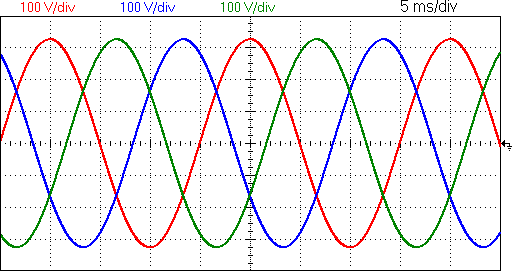
\includegraphics[width=0.5\textwidth]{images/image21001_1.png}%
\caption{Un réseau triphasé 50 Hz}%
\end{figure}

%
\linebreak%
Quelle est la tension efficace entre phases de ce réseau ?

%
\linebreak%
\begin{checkboxes}%
\CorrectChoice%
230 Volt

%
\choice%
325 Volt

%
\choice%
400 Volt

%
\choice%
460 Volt

%
\end{checkboxes}%
\linebreak%
\question{\textbf{Tableaux }}%
\textit{\textbf{Barème :} bonne réponse 4 points, mauvaise réponse-0,5 point, je ne sais pas 0 point}

%
On donne le chronogramme des tensions entre phase et neutre d'un réseau triphasé $50 Hz$ :

%
\begin{tabular}{|c|c|c|c|c|}%
\hline%
&\multicolumn{3}{|c|}{Singular}&Plural\\%
\cline{2%
-%
4}%
&Masculine&Neuter&Feminine&\\%
\hline%
Nominative&*der*&*das*&*die*&*die*\\%
Accusative&*den*&*das*&*die*&*die*\\%
Dative&*dem*&*dem*&*der*&*denen*\\%
Genitive&*dessen*&*dessen*&*deren*&*deren*\\%
\hline%
\end{tabular}%
\linebreak%
\linebreak%
Quelle est la tension efficace entre phases de ce réseau ?

%
\linebreak%
\begin{checkboxes}%
\choice%
réponse numéro $1$

%
\choice%
réponse numéro $2$

%
\CorrectChoice%
réponse numéro $3$

%
\choice%
réponse numéro $4$

%
\end{checkboxes}%
\linebreak%
\end{questions}%
\end{document}